\documentclass[11pt, oneside]{article}   	% use "amsart" instead of "article" for AMSLaTeX format
\usepackage[margin=1in]{geometry}                		% See geometry.pdf to learn the layout options. There are lots.
\geometry{letterpaper}                   		% ... or a4paper or a5paper or ... 
\usepackage{graphicx}				% Use pdf, png, jpg, or eps§ with pdflatex; use eps in DVI mode
								% TeX will automatically convert eps --> pdf in pdflatex		
\usepackage{amssymb}
\usepackage{xcolor}
\usepackage{multirow}
\usepackage{fancyhdr}
\usepackage[normalem]{ulem}
%\usepackage{substack}
\usepackage{mathtools}
\usepackage{multirow}
\usepackage{url}
%SetFonts

\newcommand{\diru}{$\uparrow$}
\newcommand{\dirl}{$\leftarrow$}
\newcommand{\dird}{$\nwarrow$}
\newcommand{\dirdl}{$\substack{\nwarrow\\\leftarrow}$}
\newcommand{\dirdu}{$\substack{\uparrow\\\nwarrow}$}
\newcommand{\dirlu}{$\substack{\uparrow\\\leftarrow}$}
\newcommand{\dirdlu}{$\substack{\uparrow\\\nwarrow\\\leftarrow}$}

\newcommand{\dirui}{\rotatebox[origin=c]{90}{$\Rsh$}}
\newcommand{\dirdi}{\rotatebox[origin=c]{90}{$\Lsh$}}
\newcommand{\diruui}{\rotatebox[origin=c]{90}{$\Rsh$}}
\newcommand{\dirdui}{$\nwarrow$\rotatebox[origin=c]{90}{$\Rsh$}}
\newcommand{\dirlui}{$\leftarrow$\rotatebox[origin=c]{90}{$\Rsh$}}
\newcommand{\dirldi}{$\leftarrow$\rotatebox[origin=c]{90}{$\Lsh$}}
\newcommand{\dirddi}{$\nwarrow$\rotatebox[origin=c]{90}{$\Lsh$}}
\newcommand{\dirudi}{$\uparrow$\rotatebox[origin=c]{90}{$\Lsh$}}
\newcommand{\dirdiui}{\rotatebox[origin=c]{90}{$\Lsh\Rsh$}}
%SetFonts


\title{Midterm Exam}
\author{CS 4364/5364}
\date{Spring 2021}							% Activate to display a given date or no date
\pagestyle{fancy}
\lhead{CS 4364/5364 Midterm}
\rhead{Spring 2021}
%\rhead{Name:\hspace{15em}}

\begin{document}
\maketitle

\paragraph{Instructions:}
Please read all of the instructions below before you begin:
\begin{itemize}
\item Read all 6 of the questions in the exam before you begin. 
\item Questions marked with a dagger (\dag) are required for students in CS 5364, and bonus (optional) for those in CS 4364
\item This document will be released to students by Midnight (12:00 am) on 11 March 2021, and will be due by 11:59pm the same day. 
\item Your submission should be sent to Dr. DeBlasio (\textbf{dan@deblasiolab.org}) by the deadline, please also send Dr. DeBlasio a private message on MS Teams (teamschat.deblasiolab.org) to inform him of your submission in case something happens with the email delivery. 
\item All submissions should be made as a single PDF file with all of your responses. 
\item All students are permitted to submit their assignments as either a typed document or as hand-written responses (scanned and clearly readable). 
\item Figured (pictograms) can be included if they help describe a solution, and are encouraged if they are clear. 
\item Remember that unanswered questions will receive 0 credit, any reasonable try at a response will receive at least half-credit. If you feel you're unable to provide a reasonable answer to a question, you can answer with ``I cannot provide a reasonable attempt for this question'', which will be provided quarter-credit. 
\item Dr. DeBlasio will have his normal office hours 1pm-2pm on test day (on teams as normal). 
\item The class period, 3-4:20pm, on the test day, will be replaced with an open question session using Zoom (the same class link).
\item Additional questions can be posed using teams private messages, but note that questions outside the times above may receive delayed responses. 
\item Monitor the `general' channel on the course team (specialtopics.deblasiolab.org/s21/teams) for errata corrections. 
\item \textbf{{\color{red}Warning:} Questions asked after 5pm on test day may not receive responses before the exam is due}.  
\end{itemize}

\clearpage
\begin{enumerate}
\item Use the \textit{Needleman-Wunch} dynamic programming table for $S = $ \texttt{CTACTGTGT} and $T = $ \texttt{CACCCCTGT} below to the next questions.
%
\renewcommand{\arraystretch}{2}
\begin{center}
{\footnotesize
\begin{tabular}{|c||c|c|c|c|c|c|c|c|c|c|c|c|}
\hline
& & \texttt{C} &  \texttt{T} &  \texttt{A} &  \texttt{C} &  \texttt{T} &  \texttt{G} &  \texttt{T} &  \texttt{G} &  \texttt{T}\\
\hline
\hline
&  0 &	  \dirl -0.5 &	 \dirl  -1 &	\dirl -1.5 &	\dirl -2 &	\dirl -2.5 &	\dirl -3 &	\dirl -3.5 &	\dirl -4 &	\dirl -4.5 \\[1ex]
\hline
\texttt{C} &  \diru -0.5 &	 \dird 5  &	 \dirl 4.5 &	\dirdl 4 &	\dirdl 3.5 &	\dirl 3 &		\dirl 2.5 &	\dirl 2 &		\dirl 1.5 &	\dirl 1 \\[1ex]
\hline 
\texttt{A} &  \diru -1 & 	\diru 4.5 & 	 \dirdlu 4 &    \dird 9.5 & \dirl 9 &		\dirl 8.5 &	\dirl 8 &		\dirl 7.5 &	\dirl 7 &		\dirl 6.5\\[1ex]
\hline
\texttt{C} &  \diru -1.5 & 	\dirlu 4 & \dirdlu 3.5 & \diru 9 &  \dird 14.5 & \dirl 14 & \dirl 13.5 & \dirl 13 & \dirl 12.5 & \dirl 12 \\[1ex]
\hline 
\texttt{C} &  \diru -2 & \dirdu 3.5 & \dirdlu 3 & \diru 8.5 &   \dirdu 14 & \dirdlu 13.5 & \dirdlu 13 & \dirdlu 12.5 & \dirdlu 12 & \dirdlu 11.5 \\[1ex]
\hline 
\texttt{C} &  \diru -2.5 & \dirdu 3 & \dirdlu 2.5 & \diru 8 &   \dirdu 13.5 & \dirdlu 13 & \dirdlu 12.5 & \dirdlu 12 & \dirdlu 11.5 & \dirdlu 11 \\[1ex]
\hline 
\texttt{C} &  \diru -3 & \dirdu 2.5 & \dirdlu 2 & \diru 7.5 &   \dirdu 13 & \dirdlu 12.5 & \dirdlu 12 & \dirdlu 11.5 & \dirdlu 11 & \dirdlu 10.5 \\[1ex]
\hline  
\texttt{T} &  \diru -3.5 & \diru 2 & \dird 7.5 & \dirlu 7 & \diru 12.5 &   \dird 18 & \dirl 17.5 & \dirdl 17 & \dirl 16.5 & \dirdl 16  \\[1ex]
\hline 
\texttt{G} &  \diru -4 & \diru 1.5 & \diru 7 & \dirdlu 6.5 & \diru 12 & \diru 17.5 &   \dird 23 & \dirl 22.5 & \dirdl 22 & \dirl 21.5 \\[1ex]
\hline 
\texttt{T} &  \diru -4.5 & \diru 1 & \dirdu 6.5 & \dirdlu 6 & \diru 11.5 & \dirdu 17 & \diru 22.5 &   \dird 28 & \dirl 27.5 & \dirdl 27 \\[1ex]
\hline 
\texttt{G} &  \diru -5 & \diru 0.5 & \diru 6 & \dirdlu 5.5 & \diru 11 & \diru 16.5 & \dirdu 22 & \diru 27.5 &  \dird 33 &  \dirl 32.5 \\[1ex]
\hline 
\end{tabular}
}
\end{center}
\begin{enumerate}
\item How many co-optimal alignments of the two strings are there? 
\item What is the optimal alignment of $S[1....3]$ and $T[1...5]$? (note these are prefixes \texttt{CTA} and \texttt{CACCC})
\item What is the mismatch penalty used to construct the table? match score? indel penalty? 
\item$^\dag$ Using \textit{only the scores in the table above} is it possible to determine the score of the optimal alignment of $S[4...9]$ and $T[6...10]$? Why or why not?
\end{enumerate}


%    \item Thinking about the posted solution for Question 2 on Homework 2, can this be adapted to
%    find a pair of non-overlapping prefixes and suffixes that maximize the total alignment score. 
%    That is a solution where $i_1 = j_1 = 1$, $i_4 = n$, $j_4 = m$.
%    Hint: since these are no longer arbitrary substrings, we will not use Smith-Waterman to find $V$ and $V'$. 
\clearpage
\item 
Use the alignments and plots below to answer the following questions:
\begin{enumerate}
\item Calculate the accuracies for the following groups of alignments, 
the reference alignment is provided at the top of each column. 
\item Given the accuracies and the parameter decompositions shown in the figures, 
what is the region of the parameter space (identify the corners of the polygon) 
that provides the best alignments on average across these two pairs of sequences. 
\end{enumerate}
Remember accuracy, with respect to a reference, is the fraction of columns from the reference that are recovered in a computed alignment; 
and that each region of the plots corresponds to a set of parameters that produce the labeled alignment.

\renewcommand{\arraystretch}{1}
\begin{center}
\begin{tabular}{r|c|r|c|}
\cline{2-2} \cline{4-4}
\multirow{2}{*}{Reference $A$} & \texttt{ATG-CTGGAT} & \multirow{2}{*}{Reference $B$} & \texttt{TTGTGTCC--}\\
& \texttt{-TGA-TCGAT} & & \texttt{TT-T-TCCAA}\\
\cline{2-2} \cline{4-4}
\multicolumn{3}{c}{}\\
\cline{2-2} \cline{4-4}
\multirow{2}{*}{$A_1$} & \texttt{ATG-CT-GGAT} & \multirow{2}{*}{$B_1$}  & \texttt{TTGTGTCC}\\
& \texttt{-TGA-TC-GAT} & & \texttt{TTTTCCAA}\\
\cline{2-2} \cline{4-4}
\multirow{2}{*}{$A_2$} & \texttt{ATGCTGGAT} &  \multirow{2}{*}{$B_2$}  & \texttt{TTGTGTCC--}\\
& \texttt{-TGATCGAT} & & \texttt{TTTT--CCAA}\\
\cline{2-2} \cline{4-4}
\multirow{2}{*}{$A_3$} & \texttt{ATG--CTGGAT} & \multirow{2}{*}{$B_3$}   & \texttt{TTGTGTCC--}\\
& \texttt{-TGATC--GAT} & & \texttt{--TTTTCCAA}\\
\cline{2-2} \cline{4-4}

\end{tabular}
\vspace{2em}

Accuracies:
\begin{tabular}{cccccc}
$A_1$ & $A_2$ & $A_3$ & $B_1$ & $B_2$ & $B_3$ \\
\hline
\multicolumn{1}{|c|}{~\hspace{3em}~} & \multicolumn{1}{|c|}{~\hspace{3em}~} & \multicolumn{1}{|c|}{~\hspace{3em}~} & \multicolumn{1}{||c|}{~\hspace{3em}~} & \multicolumn{1}{|c|}{~\hspace{3em}~} & \multicolumn{1}{|c|}{~\hspace{3em}~}\\
\multicolumn{1}{|c|}{} & \multicolumn{1}{|c|}{} & \multicolumn{1}{|c|}{} & \multicolumn{1}{||c|}{} & \multicolumn{1}{|c|}{} & \multicolumn{1}{|c|}{}\\
\multicolumn{1}{|c|}{} & \multicolumn{1}{|c|}{} & \multicolumn{1}{|c|}{} & \multicolumn{1}{||c|}{} & \multicolumn{1}{|c|}{} & \multicolumn{1}{|c|}{}\\
\hline
\end{tabular}


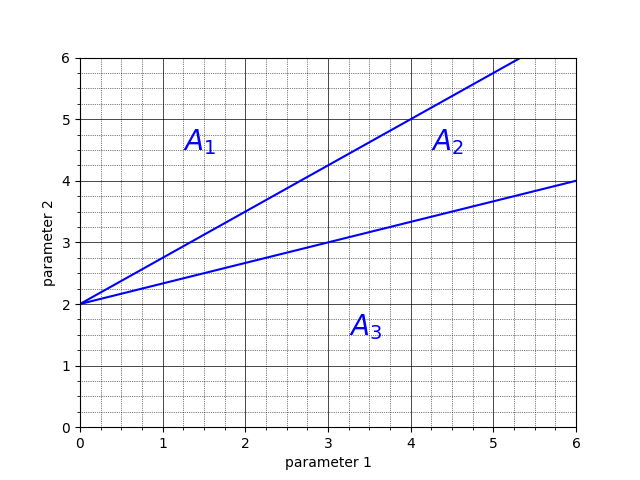
\includegraphics[width=0.46\textwidth]{Param-SpaceA}
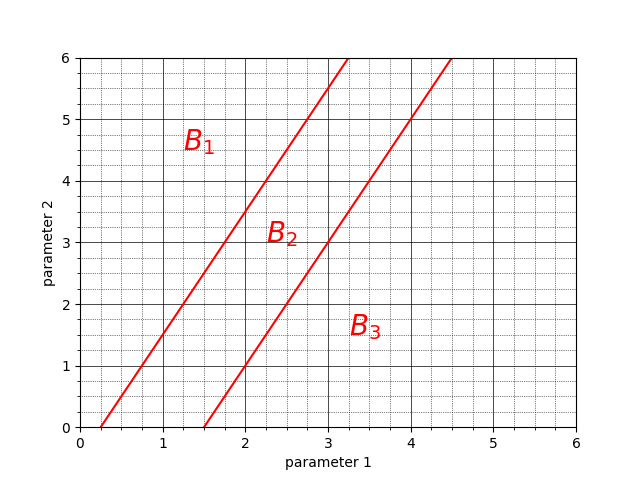
\includegraphics[width=0.46\textwidth]{Param-SpaceB}

\end{center}

\clearpage
\item Use the suffix tree below to answer the next questions. 
\label{q:SuffTree}

\begin{figure}[h!]
\centering
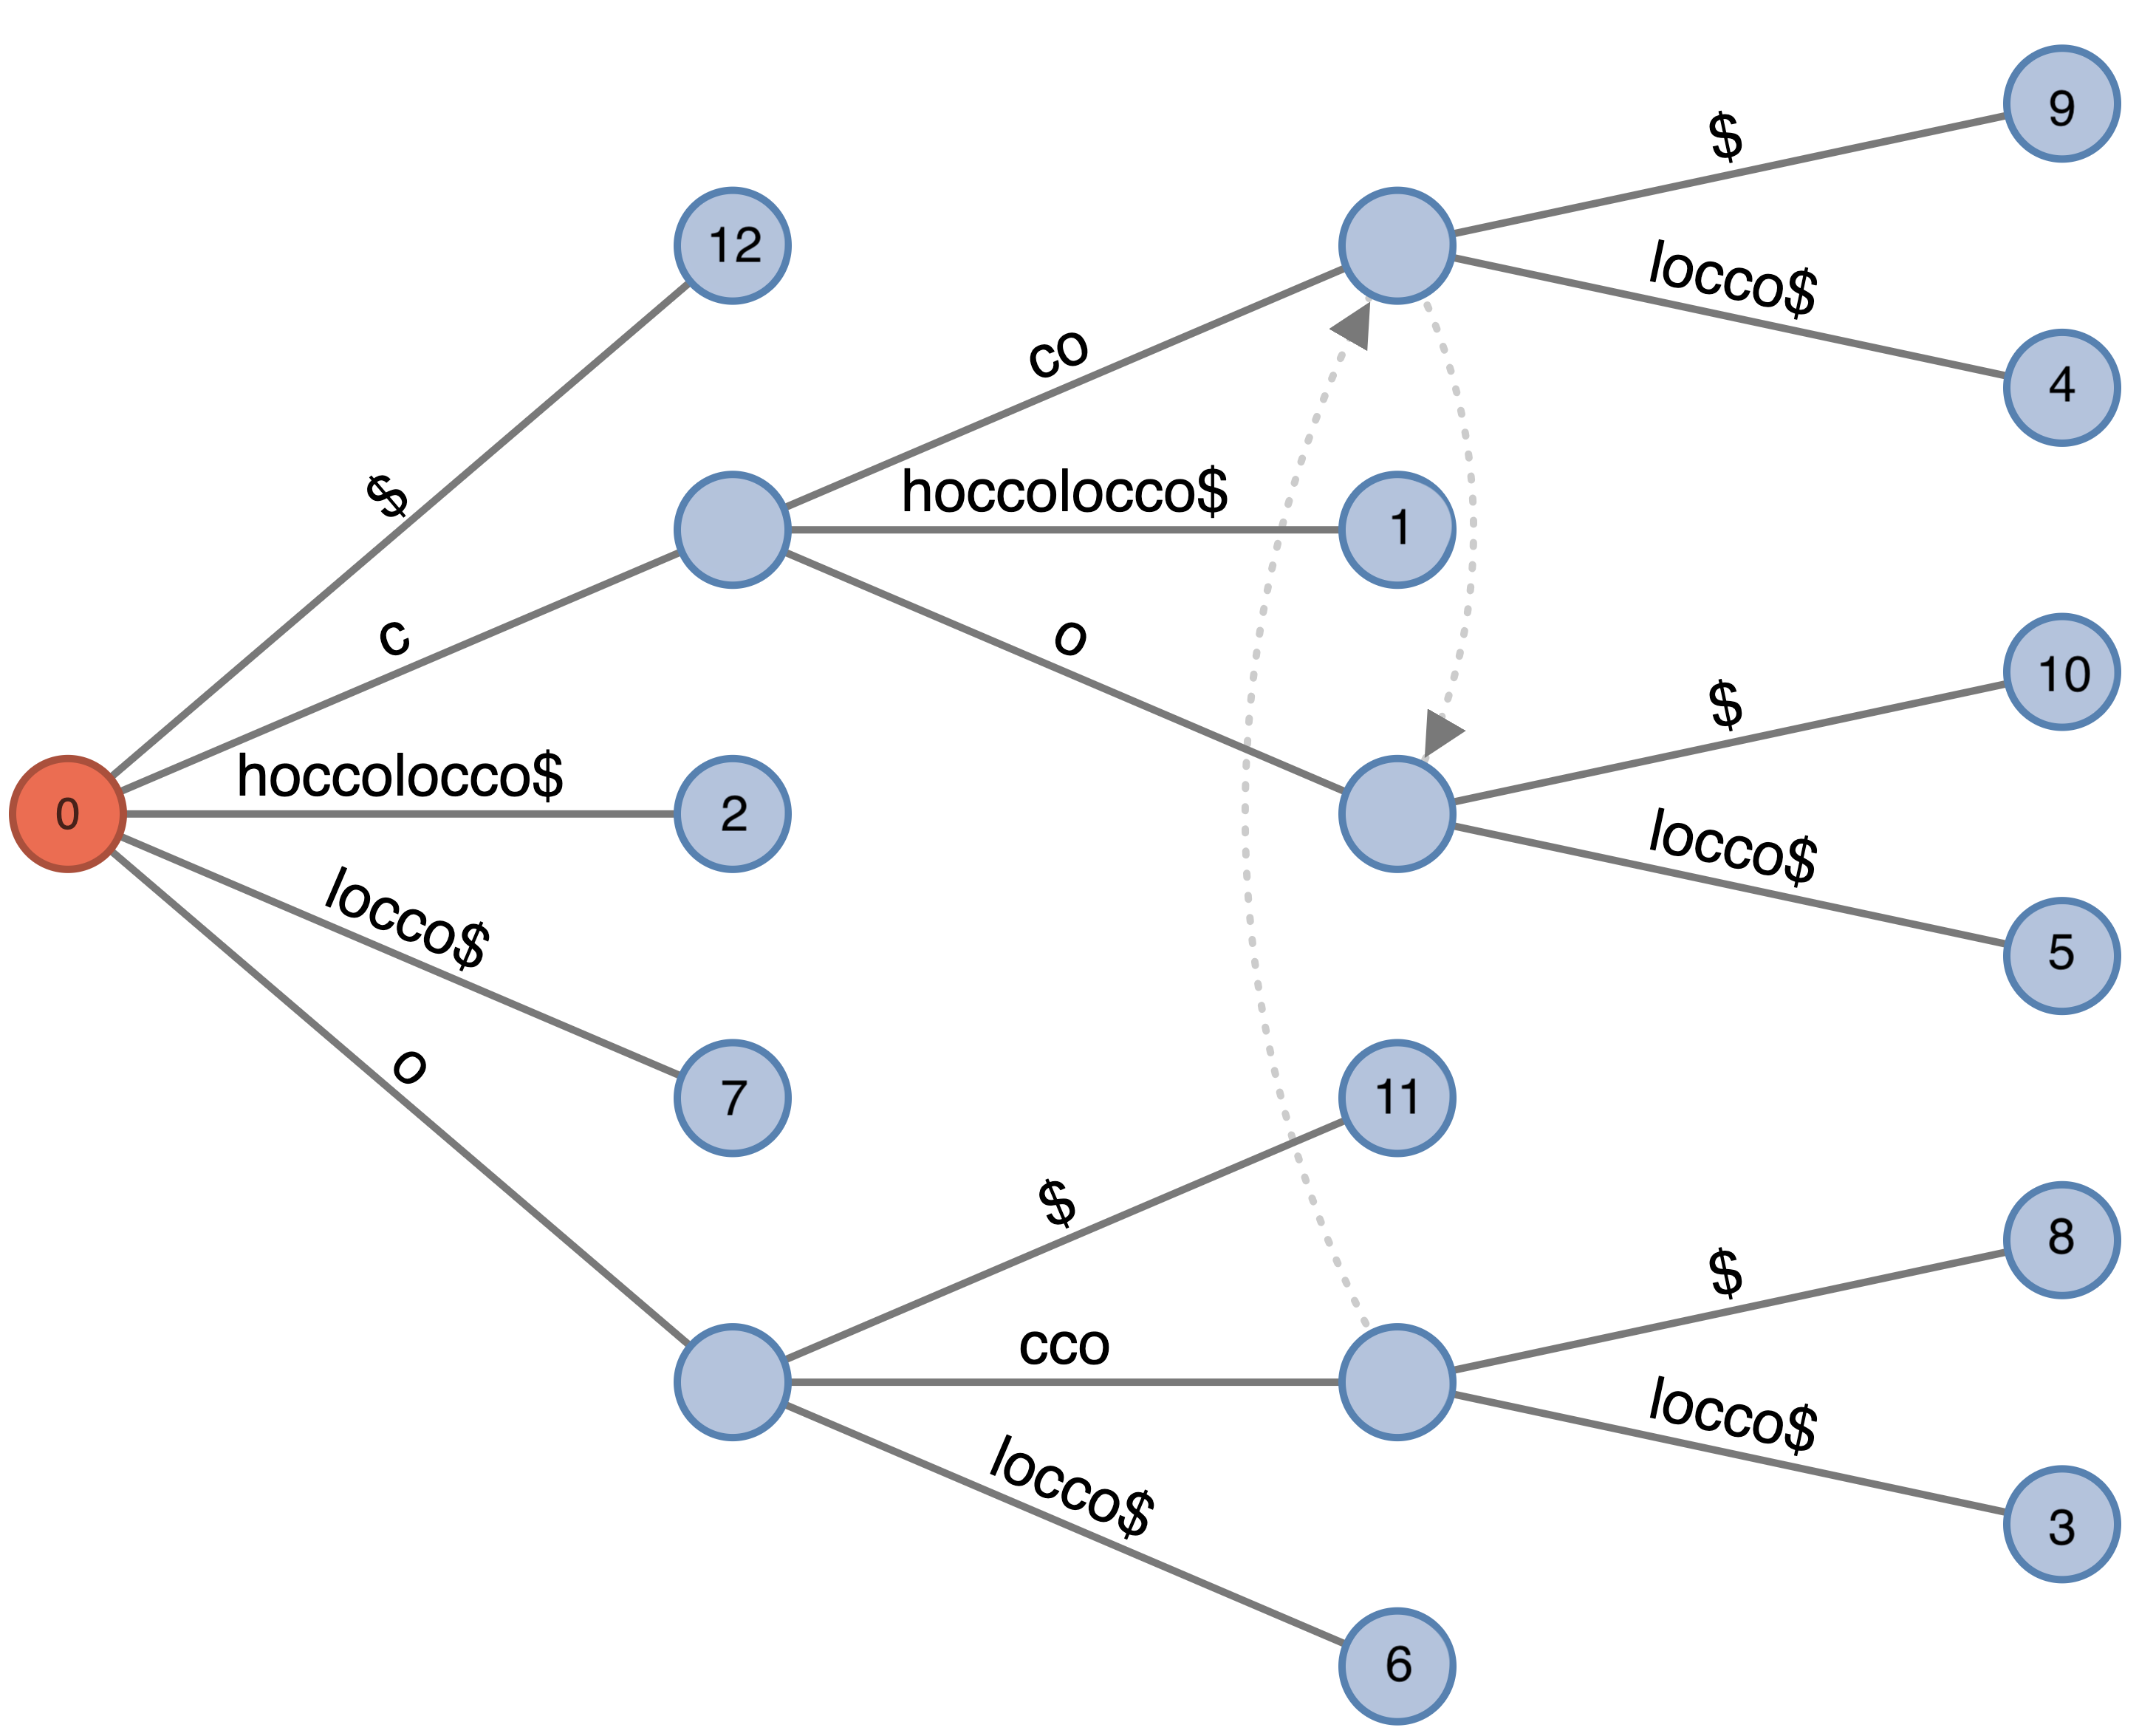
\includegraphics[width=0.75\textwidth]{midterm_ST}
\label{f:SuffTree}
\caption{Suffix tree for question~\ref{q:SuffTree}}
\end{figure}

\begin{enumerate}
\item What is the full string for which this is the suffix tree? 
\item What is the longest sub-string that occurs 2 times? 
\item What is the lexicographically smallest suffix that is strictly longer than 1 character? (that is, its more than just \texttt{\$})
\end{enumerate}



\clearpage 
\item Below is an ILP for pairwise global sequence alignment with several constraints missing. 
The scoring uses a match score of $\alpha$, a mismatch penalty of $\beta$ and an indel penalty of $\gamma$. 
Define these constraints. 
\renewcommand{\arraystretch}{2}
\begin{equation*}
\begin{array}{ll@{}ll}
\text{maximize}  & \displaystyle\alpha \sum_{i,j} X_{ij} - \beta \sum_{i,j} Y_{ij} - \gamma \left(\sum_i Z^S_i + \sum_j Z^T_j\right) \\
\text{subject to}& \displaystyle\sum_j X_{ij} + \sum_j Y_{ij} + Z^S_i  = 1 & \forall i\\
			& \text{\_\_\_\_\_\_\_\_\_\_\_\_\_\_\_\_\_\_\_\_\_\_\_\_\_\_\_\_\_\_\_\_\_\_\_\_\_\_\_\_\_\_\_\_\_\_\_\_}& \forall j\\
			& \text{\_\_\_\_\_\_\_\_\_\_\_\_\_\_\_\_\_\_\_\_\_\_\_\_\_\_\_\_\_\_\_\_\_\_\_\_\_\_\_\_\_\_\_\_\_\_\_\_}& \forall i,j: S[i] =T[j]\\
			& \text{\_\_\_\_\_\_\_\_\_\_\_\_\_\_\_\_\_\_\_\_\_\_\_\_\_\_\_\_\_\_\_\_\_\_\_\_\_\_\_\_\_\_\_\_\_\_\_\_}& \forall i,j: S[i] \ne T[j]\\
			& \text{\_\_\_\_\_\_\_\_\_\_\_\_\_\_\_\_\_\_\_\_\_\_\_\_\_\_\_\_\_\_\_\_\_\_\_\_\_\_\_\_\_\_\_\_\_\_\_\_}& \forall i < i', j > j'\\
			& X_{ij} \in \{0,1\}, & \forall i,j\\
			& Y_{ij} \in \{0,1\}, & \forall i,j\\
			& Z^S_i \in \{0,1\}, & \forall i\\
			& Z^T_j \in \{0,1\}, & \forall j\\
\end{array}
\end{equation*}
Hints: 
\begin{itemize}
\item The first constraint enforces that each position $i$ in $S$ can only be a match, a mismatch or a deletion, the second constraint will do something similar but for $T$. 
\item The 3rd and 4th constraints decide if a position is a match or mismatch, remember when defining an ILP we usually say what a value \textit{can't be} based on the information in the problem. 
\item The 5th constraint will be similar to the one we defined for LCS, but here we have two variables that can define a match between any two indexes. 
\end{itemize}

\clearpage

\item$^\dag$ True or False: When computing the sum of pairs score of a multiple sequence alignment 
 \[id + 2 mt + 2 ms = L {k\choose 2},\] 
where $id$ is the total number of indels, $ms$ is the total number of mismatches, $mt$ is the total number of matches, $k$ is the number of strings aligned, and $L$ is the length of the alignment itself. 
Justify your answer. 

\item (bonus for all) What is the item that is the answer to question~\ref{q:SuffTree}a? (You can use google for this one)

\end{enumerate}

\end{document}